\chapter[Clusters And The LSS Environment]{The Impact of the Large Scale Environment Upon Cluster Observables}

\section{Introduction}

Galaxy cluster halos are prolate spheroidal in shape, with major axes oriented
along large scale structures
\citep{CO05.1,KA05.1,BA06.1,AL06.1,AL06.2,AR07.1,BE07.1,ZH09.1,PA11.1}. Through
the study of cosmological simulations, this connection between clusters and
their environment is largely caused by the redirection of the dark matter halo
axes along the direction of the last major merger event \citep{VA93.1,SP97.1}.

It has also been well-established that cluster properties, like mass and
concentration, are highly sensitive to projection of non-spherical
distributions of mass, particularly for the various flavors of gravitational
lensing \citep{CN2007,SerenoEtAl2010b}. This effect has also 
been shown to be important in X-ray reconstructions
\citep{BU07.1,SC07.1,ET11.1}, as well as the caustic method
\citep{SV15.1}. Reconstructing the 3-dimensional mass distribution within the
cluster is currently a highly degenerate procedure, in that an infinite number
of distributions may lead to the same mass map projected on the
sky. Consequently, it becomes incredibly important to look for other clues
which may help us assign likelihood to the orientation and shape of the cluster
halos in 3-dimensional space.

Using galaxies as tracers of the large-scale structure (by means of redshift
surveys), the cluster environment can be fully mapped out in 3-dimensions and
studied alongside their 2-dimensional radial density profile properties. Since
galaxy clusters are expected to point along filaments, a strong correlation
between the orientation of the filament and the values of the concentration and
mass {\em should} exist. For an environment consistent with line-of-sight
structure, we expect to see higher cluster concentration and mass
measurements.


\section{Data}
 
In order to study the relationship between cluster observables and the
surrounding large scale structure, we require overlapping cluster and galaxy
datasets. We use the locations of spectroscopically confirmed galaxies from
Sloan Digital Sky Survey (SDSS) Data Release 10 (Fig 4.1) to trace out the large scale
structure. In total, the survey covers 14,555 square degrees of the sky, with a
magnitude limit of around 22. From this data release, we obtain the
spectroscopic redshift, right ascension, and declination measurements of just
under 1.4 million galaxies within an area on the sky defined by the following right
ascension and declination bounds: $\mathrm{100^{\circ} \le \alpha \le
  270^{\circ}}$ and $\mathrm{ -10^{\circ} \le \delta \le 70^{\circ} }$ (Fig 4.2).

Cluster concentration and mass measurements, redshifts, and their locations on
the sky, are taken from Chapter 3. It should be noted that these
measurements have been normalized over overdensity convention, cosmology, and
uncertainty convention (see Section 3.3.1). Starting with 361
unique clusters, a sub-sample of 203 is selected, based upon the constraint
that they must exist within the SDSS survey volume outlined above.

\begin{figure}
\begin{center}
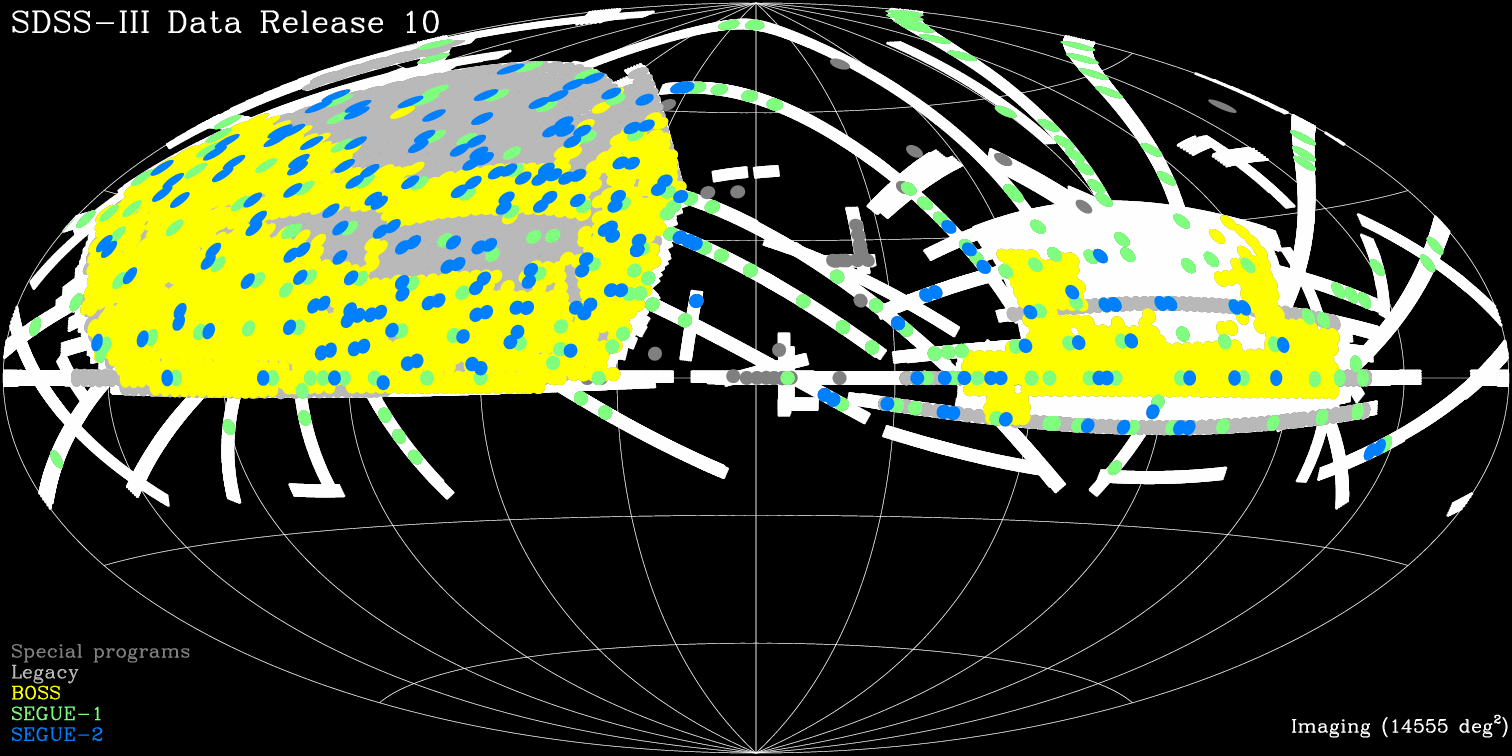
\includegraphics[width=\textwidth]{images/ClusterEnvironment/dr10_spectro_coverage.png}
\end{center}
\caption[The SDSS DR10 Footprint]{Image: www.sdss3.org. The SDSS DR10 survey
  footprint. In total, there are 1,848,851 spectroscopically confirmed galaxies
  within the dataset, out to a redshift of approximately $\mathrm{z \approx 1}$.}
\end{figure}

\begin{figure}
\begin{center}
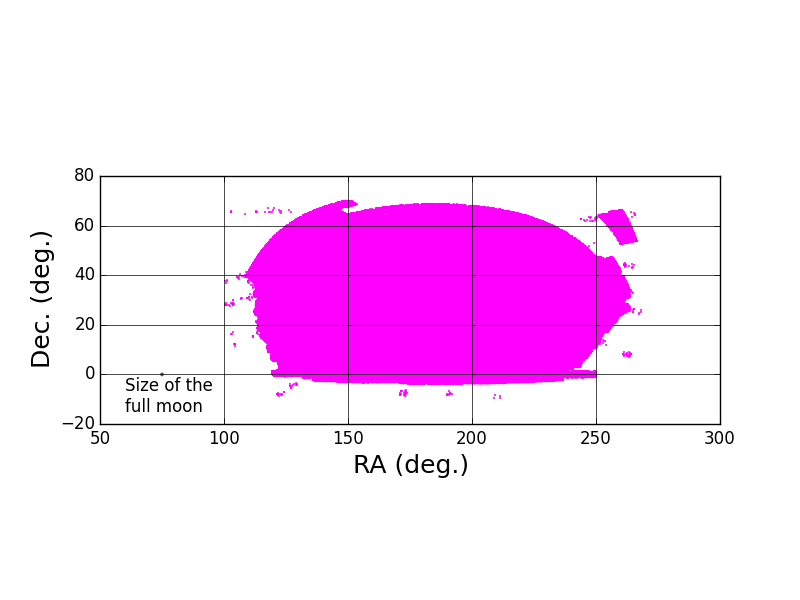
\includegraphics[width=\textwidth]{images/ClusterEnvironment/sdss_data.png}
\end{center}
\caption[The Galaxy Sample Defined]{The subset of SDSS galaxies we use for our study have been selected
  between RA $\mathrm{100^{\circ} \le \alpha \le 270^{\circ}}$, and a declination
of $\mathrm{ -10^{\circ} \le \delta \le 70^{\circ} }$.}
\end{figure}

\begin{figure}
\begin{center}$
\begin{array}{c}
  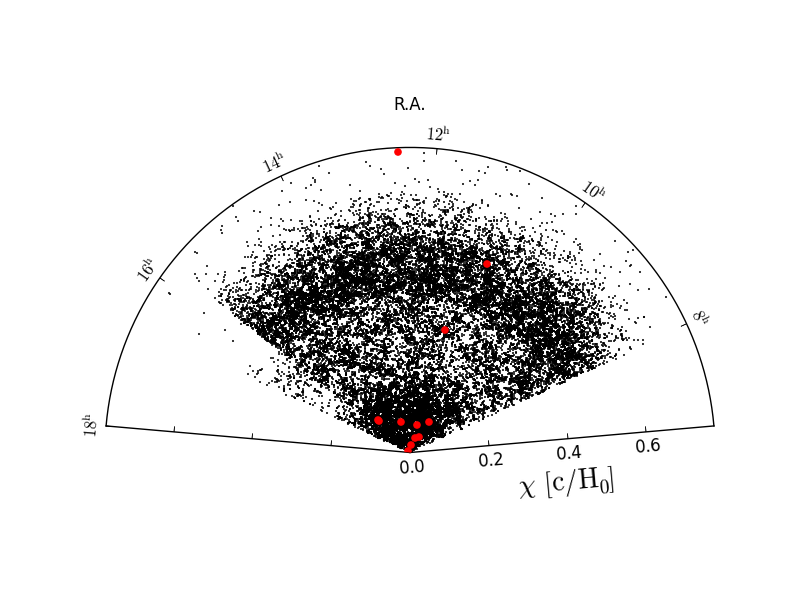
\includegraphics[width=0.9\textwidth]{images/ClusterEnvironment/sample_slice.png} \\
  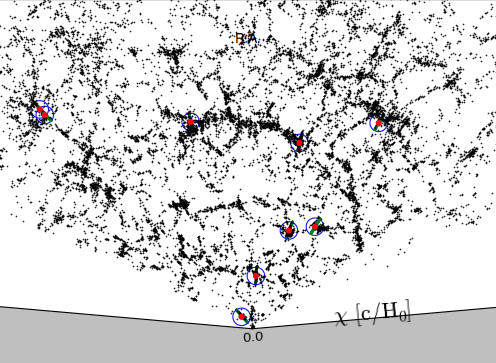
\includegraphics[width=0.85\textwidth]{images/ClusterEnvironment/sample_slice_zoom.png}
\end{array}$
\end{center}
\caption[Galaxy Clusters In SDSS]{{\em Top:} A 2 degree slice in declination of the SDSS galaxy
  population (black), with clusters (red) obtained from [CITE GR15.1]. The
  observer is located at the origin. {\em Bottom:} A blown-up version of the
  top panel, showing the filamentary-like structure of the universe. Blue
  circles give scale ($\mathrm{10 h^{-1} \, Mpc}$), and green bars show
  the line-of-sight direction at the location of each cluster.} 
\end{figure}

\section[Galaxies Around Clusters]{Obtaining Large-Scale Structure Around Clusters}
Isolating SDSS galaxies around each cluster becomes our first major step in
determining the effects of the large-scale environment upon cluster
measurements. Since cluster alignment is said to correlate with the direction
of filaments on scales up to $\mathrm{30 h^{-1} \, Mpc}$, we select an outer
radius of $\mathrm{10 h^{-1} \, Mpc}$, which is nearly an order of
magnitude larger than the outer radii of typical clusters, $\mathrm{\sim 1.5
  h^{-1} \, Mpc}$ (Fig. 4.3).

To keep the volume roughly the same around clusters at all redshifts, we use
the following condition for the association of galaxies to a given
cluster. Firstly, the spherical coordinates of the $\mathrm{i^{th}}$ cluster
are:
\begin{equation}
\mathrm{{\vv{r}}_{i} = \langle\, \chi_{i},\, \alpha_{i},\, \delta_{i}\, \rangle}
\end{equation}
where $\mathrm{\chi_{i}}$ is the comoving distance to the $\mathrm{i^{th}}$
cluster at redshift $\mathrm{z_{i}}$
\begin{equation}
\mathrm{\chi_{i} = \frac{c}{H_{0}} \int_{0}^{z_{i}}}
\frac{dz}{\sqrt{\Omega_{m,0}(1+z)^{3} + \Omega_{\Lambda}}}
\end{equation}
with the Hubble distance being $\mathrm{c/H_{0} = 3000 h^{-1}\, Mpc}$, and
where $\mathrm{\alpha_{i}}$ and $\mathrm{\delta_{i}}$ represent the right
ascension and declination of the cluster (in radians).

We then calculate the coordinates of every SDSS galaxy in the sample by placing
the $\mathrm{i^{th}}$ cluster at the origin of a new spherical coordinate
system. For the $\mathrm{j^{th}}$ galaxy, these coordinates would look like:
\begin{equation}
\mathrm{{\vv{r}}_{ij} = \langle\, {x^{1}}_{ij},\, {x^{2}}_{ij},\, {x^{3}}_{ij}\, \rangle}
\end{equation}
where
\begin{subequations}
\begin{equation}
\mathrm{{x^{1}}_{ij} = \chi_{j} - \chi_{i}}
\end{equation}    
\begin{equation}
\mathrm{{x^{2}}_{ij} = (\alpha_{j} - \alpha_{i}) \cos \delta_{i} \, D_{A,i}}
\end{equation}
\begin{equation}
\mathrm{{x^{3}}_{ij} = (\delta_{j} - \delta_{i}) \, D_{A,i}}
\end{equation}
\end{subequations}
A new distance measure is introduced here, the angular diameter distance,
$\mathrm{D_{A}}$, which is defined in terms of the comoving distance,
$\mathrm{\chi}$.
\begin{equation}
\mathrm{D_{A} = \frac{\chi}{1+z}}
\end{equation}
Selecting galaxies within a radius of $\mathrm{R = 10 h^{-1}\, Mpc}$ becomes a
straightforward condition to check:
\begin{equation}
\mathrm{({x^{1}}_{ij})^{2} + ({x^{2}}_{ij})^{2} +  ({x^{3}}_{ij})^{2} \le R^{2}} 
\end{equation}

As an example of this procedure, Figure 4.4 shows SDSS galaxies selected around
the cluster Abell 1238.

\begin{figure}
\begin{center}
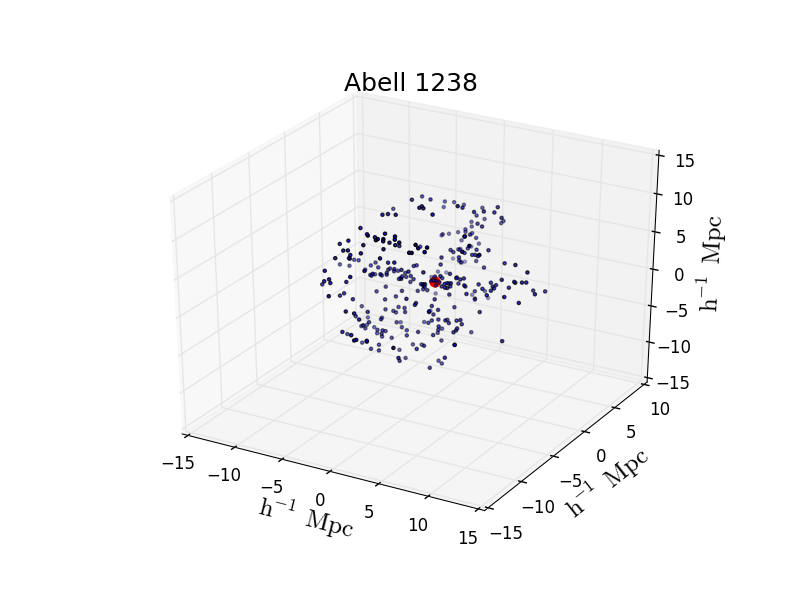
\includegraphics[width=\textwidth]{images/ClusterEnvironment/Abell1238.png}
\end{center}
\caption[Selecting Galaxies Around Clusters]{Shown here are the 322 spectroscopically confirmed SDSS galaxies
  (black scatter points) around the galaxy cluster Abell 1238 (red), located at a
  redshift of $\mathrm{z=0.0733}$.}
\end{figure}

Lastly, we enforce a threshold of $\mathrm{N_{gal} \ge 100}$ in order to ensure
that only clusters with a sufficiently dense tracing of its environment are
used for further study. This cuts our sample from 203 unique clusters down to 92.

\subsection{Quantifying Structure}
We are looking to understand if line-of-sight large-scale structure has an
impact on cluster concentration and mass measurements. Our first attempt at
quantifying the structures we find around clusters is to focus on the
distributions of azimuthal ($\mathrm{\theta}$) and polar ($\mathrm{\phi}$)
angles.
 \begin{subequations}
\begin{equation}
\mathrm{\theta = \tan^{-1} \left( \frac{y}{x} \right)}
\end{equation}    
\begin{equation}
\mathrm{\phi = \cos^{-1} \left( \frac{z}{r} \right)}
\end{equation}
\end{subequations}
where we define $\mathrm{ \{ x\equiv x^{2},\, y\equiv x^{3},\, z\equiv x^{1}
    \} }$, and where $\mathrm{r = \sqrt{(x^{1})^{2} + (x^{2})^{2} +
    (x^{3})^{2}}}$.

From these angles, we can make use of spherical harmonic functions, which
are commonly used special functions defined on the surface of a sphere. Due to
their orthogonal nature, any arbitrary angular function can be expressed
as a linear combination of spherical harmonics.
\begin{equation}
\mathrm{f(\theta,\phi) = \sum_{l=0}^{\infty} \sum_{m=0}^{l} A_{l}^{m}
  Y_{l}^{m} (\theta,\phi)}
\end{equation}

Spherical harmonics are defined by a set of integers, $\mathrm{l}$ and
$\mathrm{m}$ ($\mathrm{m=-l,...l}$), roughly corresponding to the shape of the
function and the orientation of the function, respectively.

The coefficients of this series can then generally be computed as follows:
\begin{equation}
\mathrm{A_{l}^{m} = \int_{0}^{2\pi}\int_{0}^{\pi} f(\theta,\phi)
  \tilde{Y_{l}^{m}}(\theta,\phi) \sin \theta\, d\theta\, d\phi}
\end{equation}
where $\mathrm{\tilde{Y_{l}^{m}}(\theta,\phi)}$ is the complex conjugate of the spherical
harmonic function, $\mathrm{Y_{l}^{m}(\theta,\phi)}$.

However, in our case, the function $\mathrm{f(\theta,\phi)}$ is discrete rather
than continuous, leading us to compute coefficients in the following way:
\begin{equation}
\mathrm{A_{l}^{m} = \frac{4\pi}{N} \sum_{i=1}^{N_{gal}} \tilde{Y_{l}^{m}}(\theta_{i},\phi_{i})}
\end{equation}

Since we expect roughly triaxial or filamentary-like large-scale structure, we pay
specific attention to the modes $\mathrm{ \{ l=1,m=-1,0,1 \}}$. 

 \begin{subequations}
\begin{equation}
\mathrm{Y_{1}^{1} = -\sqrt{\frac{3}{8\pi}} \sin \theta \,e^{i\phi}}
\end{equation}    
\begin{equation}
\mathrm{Y_{1}^{0} = \sqrt{\frac{3}{4\pi}} \cos \theta}
\end{equation}
\begin{equation}
\mathrm{Y_{1}^{-1} = \sqrt{\frac{3}{8\pi}} \sin \theta \,e^{-i\phi}}
\end{equation}
\end{subequations}


These spherical harmonics 
give us an idea about the elongation
of structure along the primary axes. Most importantly is the value of
$\mathrm{A_{1}^{0}}$ (line-of-sight direction, z) relative to
$\mathrm{A_{1}^{1}}$  and $\mathrm{A_{1}^{-1}}$ (in x- and
y-directions, respectively).  From these coefficients, the statistic we compute
is:
\begin{equation}
\mathrm{\frac{A_{1}^{0}}{\sqrt{{A_{1}^{0}}^{2}+{A_{1}^{0}}^{2}}}}
\end{equation}


\section{Results And Future Work}

In this section, we present the results of our correlation tests between the
line-of-sight statistic (4.12), with cluster mass $\mathrm{M_{vir}}$ (Figure 4.5),
concentration $\mathrm{c_{vir}}$ (Figure 4.6),  and the redshift-scaled concentration
$\mathrm{c_{vir}(1+z)}$ (Figure 4.7). In all cases, we find no discernable correlation
between cluster observables and line-of-sight orientation of its surrounding
environment on scales of up to $\mathrm{10 h^{-1} Mpc}$. In each figure, we
also highlight clusters which contain measurements which were made with weak
lensing.

With a sample size of 92 clusters, it is difficult for us to completely reject the
idea that angular information about galaxies around clusters (out to sufficient
distances) {\em can} tell us about the true inclination of clusters with
respect to the line-of-sight. Keeping this in mind, characterizing the
large-scale galaxy distribution is made in a number of ways, many of
which we have not yet attempted with our sample. Including radial information
may prove useful, however, we would truly benefit the most by having a much
larger cluster sample (for instance, the maxBCG sample \citealt{KO07.1}, which
contains 13,823 galaxies found within SDSS).

The breakdown by method of cluster concentrations and masses measured for our
92 clusters are the following (remembering that some clusters are measured
multiple times): 
\begin{itemize}
\item LOSVD: 34 
\item CM: 62
\item X-ray: 33
\item WL: 5
\end{itemize}

Redshift-based distance measurements of galaxies are
sensitive to two general effects, arising from their peculiar velocities
(additional motion which is not defined by the Hubble flow). The first effect is
called the ``finger of God'' effect, whereby distances to galaxies are over-estimated
(under-estimated) due to their radial motion away from (toward) the observer
while orbiting within the cluster. This effect becomes important once typical
peculiar velocities for galaxies around clusters ($\mathrm{v_{pec} \approx 300
  \, km/s}$) are comparable to their recession speed due to the expansion of the
universe ($\mathrm{v_{exp} = cz}$ for relatively low redshifts). Nearby
clusters suffer an elongation of their structure along the direction of
observation. A much smaller effect than the ``finger of God'' effect, entitled
the Kaiser effect, is caused by the coherent motions of galaxies as they fall
toward clusters as they assemble. Instead of an elongation along the
line-of-sight, structures are flattened perpendicular to this direction,
creating pancake-like structures. Their combined effects are 
seen in the correlation function of galaxies in surveys like the two degree
field galaxy redshift survey (2dfGRS) \citep{HA03.1}. Redshift space
distortions become important once the distributions around clusters are
quantified in any way. Careful subtraction of cluster members is therefore the
only way to mitigate these effects upon our final result. In order to do this
however, we require catalogs of cluster members.

\begin{figure}
\begin{center}
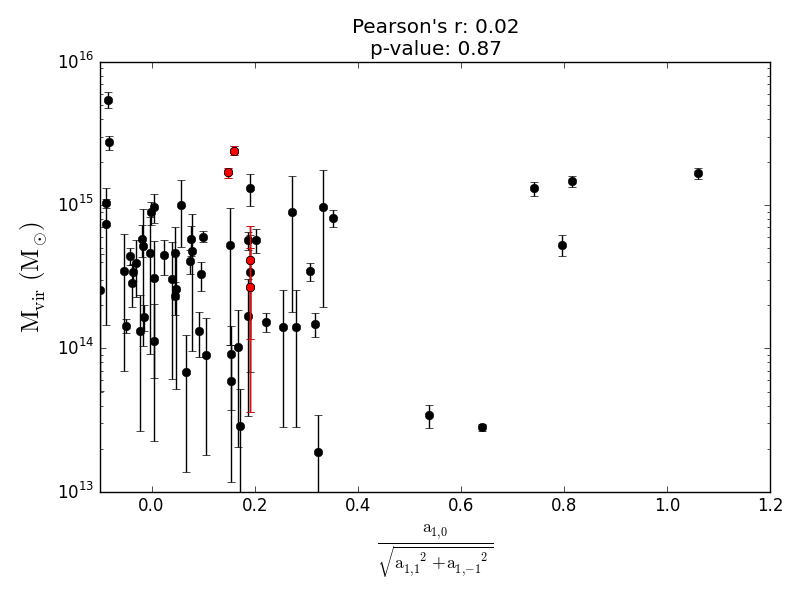
\includegraphics[width=\textwidth]{images/ClusterEnvironment/Mass_Corr2.png}
\end{center}
\caption[Mass - $\mathrm{A_{l}^{m}}$ Correlation]{The correlation between the total
cluster halo mass, $\mathrm{M_{vir}}$, and the measure of line-of-sight
orientation of environmental structure using the spherical harmonic
coefficients, $\mathrm{A_{l}^{m}}$. Larger values indicate more line-of-sight
structure relative to perpendicular structure. Red points indicate clusters
which make use of weak lensing (WL) measurements.}
\end{figure}

\begin{figure}
\begin{center}
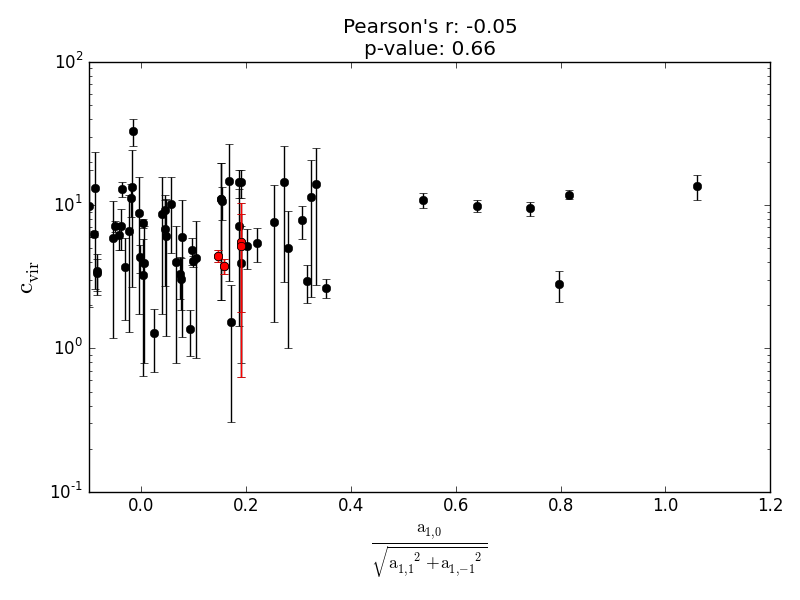
\includegraphics[width=\textwidth]{images/ClusterEnvironment/Conc_Corr2.png}
\end{center}
\caption[Concentration - $\mathrm{A_{l}^{m}}$ Correlation]{The correlation
  between the cluster concentration, $\mathrm{c_{vir}}$, and the measure of
  line-of-sight orientation of environmental structure using the spherical
  harmonic coefficients, $\mathrm{A_{l}^{m}}$. Larger values indicate more
  line-of-sight structure relative to perpendicular structure. Red points indicate clusters
which make use of weak lensing (WL) measurements.}
\end{figure}

\begin{figure}
\begin{center}
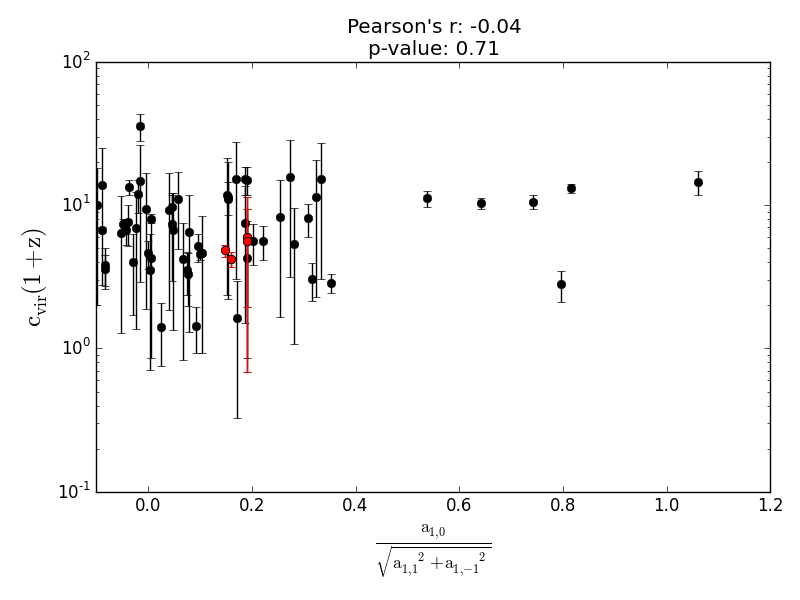
\includegraphics[width=\textwidth]{images/ClusterEnvironment/ConcRedshift_Corr2.png}
\end{center}
\caption[Redshift Scaled Concentration - $\mathrm{A_{l}^{m}}$ Correlation]{The
  correlation between the redshift-scaled cluster concentration,
  $\mathrm{c_{vir}(1+z)}$, and the measure of line-of-sight orientation of
  environmental structure using the spherical harmonic coefficients,
  $\mathrm{A_{l}^{m}}$. Larger values indicate more line-of-sight structure
  relative to perpendicular structure. Red points indicate clusters
which make use of weak lensing (WL) measurements.}
\end{figure}